% ----------------------------------------------------------
\chapter{Experiments and Results}\label{ch:experiments}
% ----------------------------------------------------------

Given the theoretical foundations exposed above, in this chapter, the proposed approach to achieve this thesis' goal is presented.
Furthermore, this approach named \gls{PIDEQ} is validated through a set of experiments, aiming to explore its performance and the impact of the many different features of the model.

\section{Problem Definition}

The Van der Pol oscillator (sec. \ref{sec:vdp}) was chosen as the \gls{ODE} system for which an \gls{IVP} will be solved.
This system is known for having no analytical solution, thus becoming a benchmark for solvers.
As well, textcite[REFTO Antonello, 2021] have already studied a solution using \gls{PINN}s, which is used as a starting point and a reference in performance for the experiments.

More specifically, we define the first-order formulation of the Van der Pol oscillator (as presented in equation \eqref{eq:vdp}) as the \gls{ODE} system, with $\mu=1$.
Then, the \gls{IVP} is defined with initial condition $\bm{y}(0) = \bm{y}_0 = \left( 0, 0.1 \right) $, simulating a small perturbation of the system at the unstable equilibrium at the origin, and the solution is desired for a horizon of 2 seconds. 
This way, the expected solution is expected to gravitate to a limit cycle, but not within the solution interval, as illustrated in figure \ref{fig:vdp_example}.

\subsection{Evaluation Metrics}

As there is no analytical solution to the \gls{IVP} at hand, the solutions will be evaluated in comparison to the approximation found using \gls{RK4}.
This reference was generated from 1000 points equally spaced in the solution interval $I=[0,2]$, with a time step of 2\,ms\footnotemark.
\footnotetext{Of course, this set does not include the initial condition, which is already given, which means that the first point of evaluation is at $t=0.002$.}
Then, a solution's approximation to the reference is measured through the \gls{IAE}, which can be defined here as \[
    IAE = \frac{1}{h}\sum_{i=1}^{1000} \|\bm{y}_i - \hat{\bm{y}}_i\|
,\] where $\bm{y}_i$ are the points in the \gls{RK4} solution,  $\hat{\bm{y}}_i$ are the points in the solution being evaluated, and $h=0.002$ is the time step.
Therefore, a solution is said proper to the problem if it achieves a low \gls{IAE}.

Besides the quality of the approximation, the time required to achieve such approximation is also of interest, as many applications (e.g., model predictive control) are highly time-dependent.
As well, the hardware resources used are valuable metrics, as the computing power necessary limits the range of equipment that can support a given solution.
These will be auxiliary to the \gls{IAE} in the analysis of the approximations.

\section{PIDEQ}

As already discussed in section \ref{sec:pinn-problem}, solving \gls{IVP}s is (mostly) only reasonable if using a physics-informed approach, that is, if "teaching" the model through the known dynamics instead of through actual samples of the target function.
Therefore, a reasonable solution using \gls{DEQ}s must follow the same principle, which implies in a physics-informed training of \gls{DEQ}s (thus, \gls{PIDEQ}).

For the \gls{IVP} defined above, we recall the definition of section \ref{sec:deq-definition} and propose a \gls{DEQ} similar to textcite[REFTO Ghaoui, 2019], that is, a model
\begin{align*}
    D_{\gls{param}}^{EQ}: \R &\longrightarrow \R^2 \\
    t &\longmapsto D_{\gls{param}}(t) = \hat{\bm{y}}
\end{align*}
such that
\begin{equation}
\begin{split}
    D^{EQ}_{\gls{param}}(t) &= C\bm{z}^{\star} \\
    \bm{z}^{\star} &= \bm{f}_{\gls{param}}\left( t,\bm{z}^{\star} \right) \\
    \bm{f}_{\gls{param}}\left( t,\bm{z} \right) &= \tanh \left( A\bm{z} + t\bm{a} + \bm{b} \right)
\end{split}
,\end{equation}
in which the parameters \gls{param} are a vectorization of the matrices and vectors, i.e., $\gls{param} = \left( A,C,\bm{a},\bm{b} \right)$, and the hyperbolic tangent function is applied to each element of the resulting vector.

Notice that this formulation is very close to the one used in chapter \ref{ch:deq}, except for the linear transformation of the equilibrium point at the model's output.
This implies that both forward and backward operations can occur in the same way, except that the term  \[
    \frac{d D^{EQ}_{\gls{param}}}{d \bm{z}^{\star}} = C^T
\] must be multiplied in the computation of the gradients.
The advantage of this modification is that we can $\bm{z}$ with an arbitrary dimension, which results in arbitrary representational power [REFTO Ghaoui, 2019].

The challenge in physics-informing a \gls{DEQ} is to optimize a cost function on its derivatives.
As it was shown in section \ref{sec:deq-backward}, textcite[REFTO Bai, 2019] have proposed an efficient way to compute the first derivative of a \gls{DEQ} with regards to either its parameters or the input, which allows us to compute the cost function value.
Yet, an application of gradient descent with such cost function, it is required that the second derivatives of the model (with respect to the input and the parameters) are computable a training time.
In practice, this implies in the computation of the derivative of the root-finding algorithm used to compute the first derivative, as seen in section \ref{sec:deq-backward-implementation}.\footnotemark
\footnotetext{In theory, it could be possible to use the implicit function theorem once again to achieve an analytical formula for the second derivative, but this is left for future work.}
This restricts us to using differentiable root-finding algorithms to compute the first derivative, relying on automatic differentiation tools to compute the second derivative.

Finally, we propose to use a cost function for training a \gls{PIDEQ} model of the form \[
    J\left( \gls{param} \right) = J_b\left( \gls{param} \right) + \lambda J_{\mathcal{N}}\left( \gls{param} \right) + \kappa \left\lVert \frac{d \bm{f}_{\gls{param}}}{d \bm{z}}\right\rVert_F
,\] 
in which $J_b$, $J_{\mathcal{N}}$ and $\lambda$ are as defined in section \ref{sec:PI}, while $\left\lVert \frac{d \bm{f}_{\gls{param}}}{d \bm{z}}\right\rVert_F$ is the Frobenius norm of the Jacobian of the equilibrium function, as exposed in sec. \ref{sec:deq-jac-reg}, a regularization term weighted by $\kappa \in \R^+$.
This cost function ensures the physics-informed training from \gls{PINN}s with the regularization term which was shown essential to \gls{DEQ}s.

\section{Training}

Early experiments helped to define the design choices for the training algorithm and the hyperparameters.
Adam[REFTO Adam paper] was the optimizer of choice, with $\gls{lr}=0.001$ and default configuration.
The loss weighting coefficients were initially set as $\lambda=0.1$ and $\kappa=1.0$.
The solver used for the forward pass of the model was the Anderson Acceleration[REFTO Walker, 2011], while best results were found using simple iteration to compute the backward pass.
% \footnotetext{More complex solvers, even if made differentiable for the automatic differentiability package, had such an increased cost for computing the second derivative that the simple iteration became a much better choice.}
For both algorithms, the tolerance was set as $\epsilon=10^{-4}$ and they were limited to 200 iterations.
The initial guess was always $\bm{z}_0=\bm{0}$.

In regard to the data, $X_b$, of course, contained only the initial condition, while $X_{\mathcal{N}}$ contained $10^5$ random samples within $I$.
The regularization term $\left\lVert \frac{d \bm{f}_{\gls{param}}}{d \bm{z}}\right\rVert_F$ was computed on the input values of both data sets.

\section{Experiments}

The experiments reported below concern the training of the deep learning model proposed above to solve the \gls{IVP} described in the first section of this chapter.
The implementation was done using PyTorch [REFTO Paszke, 2019] and is available at \url{https://github.com/brunompacheco/pideq}.
All experiments were performed on a high-end computer, using an RTX 3060 GPU.
A budget of 50000 epochs was chosen.
% TODO add number of runs

\subsection{Baseline Results}

The baseline result for a \gls{PINN} trained to solve an \gls{IVP} of the Van der Pol oscillator comes from textcite[REFTO Antonello, 2021].
We replicate these results, that is, a traditional \gls{PINN} with 4 hidden layers with 20 nodes each, following the same setup proposed above (except for the regularization term of the cost function).
At the same time, textcite[REFTO Ghaoui, 2019] showed that a \gls{DEQ} with $\bm{z}$ containing as many dimensions as there are hidden nodes in a given deep feedforward network, has \emph{at least} as much representational power as that network.
Then, our starting \gls{DEQ} is a model with  $\bm{z}\in \R^{80}$.

The results for both models can be seen in figure XXX.
Given that the \gls{PINN} used was able to "learn" (i.e., to achieve a low IAE on) the task, we expect that the large \gls{DEQ} model also is capable of learning.

\begin{figure}[h]
    \centering
	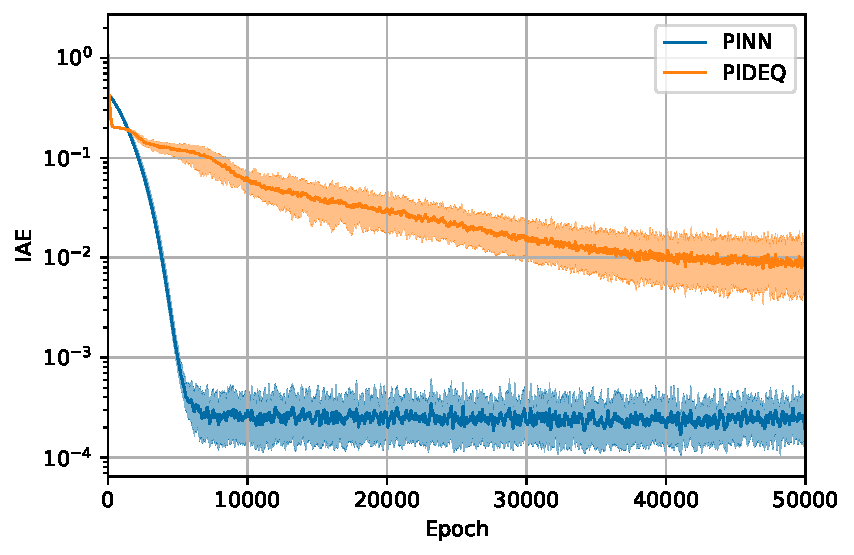
\includegraphics{images/exp_1_iae.pdf}
    \caption{Learning curve for the baseline models trained on the \gls{IVP} for the Van der Pol oscillator.}
    \label{fig:images-exp_1_iae-pdf}
\end{figure}

- Antonelo trained a PINN to solve this exact same problem with 4x20
- we replicate this results
- theoretical baseline is that a DEQ has at least as much representational power as a net with the same amount of nodes in total, so a DEQ with 80 states should be able to learn the task
- show results

\subsection{Number of States}

- show sparse matrix and how it points out to a smaller model
- process repeated
- while a 5 states DEQ can learn the task, it takes longer to converge


